% section3_1_posterior.tex — Module B: Bo
% Addresses QHM Core Task 1, §3.3 (MCMC Sampling).
\subsection{Posterior Inference}\label{sec:posterior}

The likelihood of Section~\ref{sec:likelihood} together with the priors of Section~\ref{sec:prior} defines a four-dimensional joint posterior distribution over $(\beta_0,\, \beta_1,\, \beta_2,\, \sigma)$ that does not admit a closed-form expression. Although a single regression coefficient with known noise variance enjoys Normal--Normal conjugacy, the joint posterior in our setting involves three coefficients alongside an unknown residual standard deviation, leaving the marginal likelihood $p(\mathbf{y})$ analytically intractable. We therefore approximate the posterior by Markov Chain Monte Carlo (MCMC) sampling, exploiting the standard property that arbitrary posterior expectations can be estimated as sample means of the resulting parameter trajectories.

\subsubsection{MCMC Sampler Configuration}

Sampling was performed with the No-U-Turn Sampler (NUTS), a self-tuning variant of Hamiltonian Monte Carlo implemented in \texttt{PyMC}~5. NUTS exploits gradient information of the log posterior to propose distant, high-acceptance moves and is widely regarded as the default choice for continuous models of this dimensionality.

We ran four independent chains, each initialised at a randomly perturbed starting point. Each chain used $1000$ warm-up iterations followed by $2000$ retained iterations, yielding a total of $8000$ posterior samples on which all subsequent inference is based. The warm-up phase serves a dual purpose: NUTS adapts its step size and the diagonal mass matrix during this phase, and the corresponding samples — which are drawn before the chain has fully entered the high-density region of the posterior — are simultaneously discarded as burn-in. We therefore retain no further explicit burn-in beyond the warm-up. The target acceptance probability was set to $0.95$, slightly above the default of $0.80$, which reduces the incidence of divergent transitions in the underlying Hamiltonian dynamics; in our run no divergent transitions were reported by the sampler. The random seed was fixed at $42$, matching the data subsampling seed used by Module~A, so that the entire pipeline is exactly reproducible from raw data to posterior summaries.

\subsubsection{Convergence Diagnostics}

Standard convergence diagnostics indicate that the four chains have converged to the same posterior distribution and that the effective sample size is sufficient for stable inference of posterior means and 95\% credible intervals. The potential scale reduction factor $\hat{R}$ equals $1.00$ for every parameter, well below the conventional threshold of $1.01$ that would signal possible non-convergence. The bulk effective sample size ranges from $3{,}775$ for $\beta_0$ to $5{,}371$ for $\beta_1$, all of which substantially exceed the rule-of-thumb minimum of $400$ recommended for stable estimation of central tendency. A more detailed treatment of trace plots, autocorrelation, and burn-in choice is presented by Module~C in Section~\ref{sec:sampler}; the present section confines itself to reporting that the diagnostics support unimpeded use of the posterior samples for inference.

\subsubsection{Posterior Summaries}

Table~\ref{tab:posterior} reports the posterior mean, posterior standard deviation, and 95\% highest-density credible interval (HDI) for each parameter, together with the convergence diagnostics. The HDI is preferred over an equal-tailed interval because it always contains the most plausible parameter values and remains meaningful for asymmetric posteriors.

\begin{table}[htbp]
\centering
\caption{Posterior summaries based on $8000$ NUTS samples ($4$ chains $\times\ 2000$ retained draws). All $\hat{R}$ values are at the convergence floor of $1.00$, and all bulk effective sample sizes exceed $3{,}500$.}
\label{tab:posterior}
\begin{tabular}{lrrrrrr}
\hline
Parameter & Mean & SD & 95\% CrI lower & 95\% CrI upper & ESS bulk & $\hat{R}$ \\
\hline
$\beta_0$ (intercept)     & $2541$  & $382$ & $1799$  & $3324$  & $3{,}775$ & $1.00$ \\
$\beta_1$ (\texttt{temp}) & $6784$  & $436$ & $5915$  & $7632$  & $5{,}371$ & $1.00$ \\
$\beta_2$ (\texttt{hum})  & $-2350$ & $555$ & $-3457$ & $-1276$ & $4{,}181$ & $1.00$ \\
$\sigma$                  & $1500$  & $\phantom{0}56$ & $1393$  & $1610$  & $5{,}352$ & $1.00$ \\
\hline
\end{tabular}
\end{table}

The marginal posterior densities of all four parameters are shown in Figure~\ref{fig:post_density}; each is approximately symmetric and unimodal, with the 95\% HDI annotated below the curve. Figure~\ref{fig:forest} provides a side-by-side comparison of the four credible intervals via a forest plot. The credible intervals for $\beta_1$ and $\beta_2$ lie wholly on opposite sides of zero, and the interval for $\sigma$ is so narrow that it is reduced to a near-point on the common scale of the plot, reflecting the high precision with which the residual scale is estimated.

\begin{figure}[htbp]
    \centering
    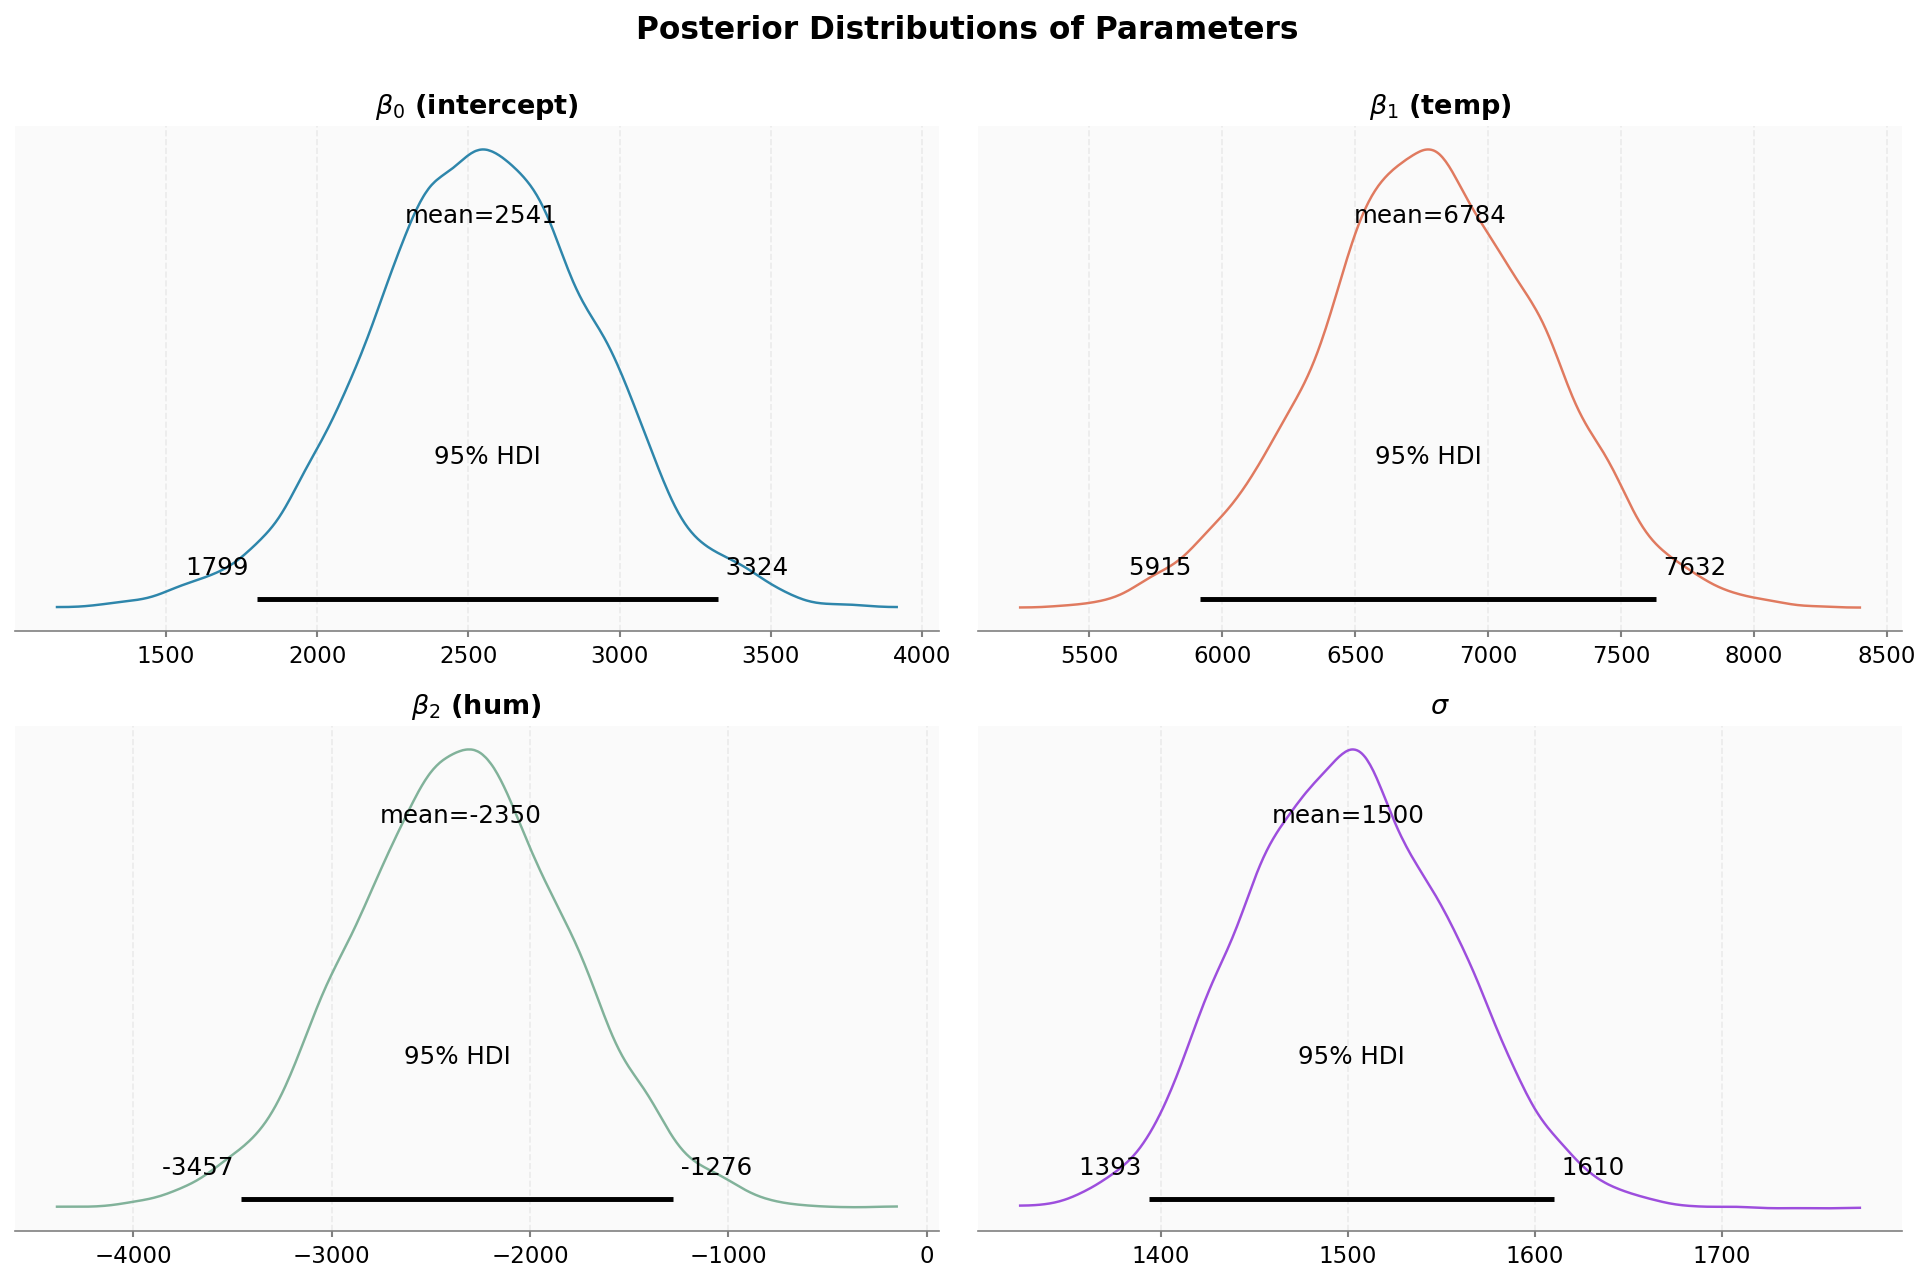
\includegraphics[width=0.85\textwidth]{../results/figures/posterior_density.png}
    \caption{Marginal posterior densities of $\beta_0$, $\beta_1$, $\beta_2$, and $\sigma$. The bar beneath each curve marks the 95\% highest-density interval; the annotated mean is the posterior mean.}
    \label{fig:post_density}
\end{figure}

\begin{figure}[htbp]
    \centering
    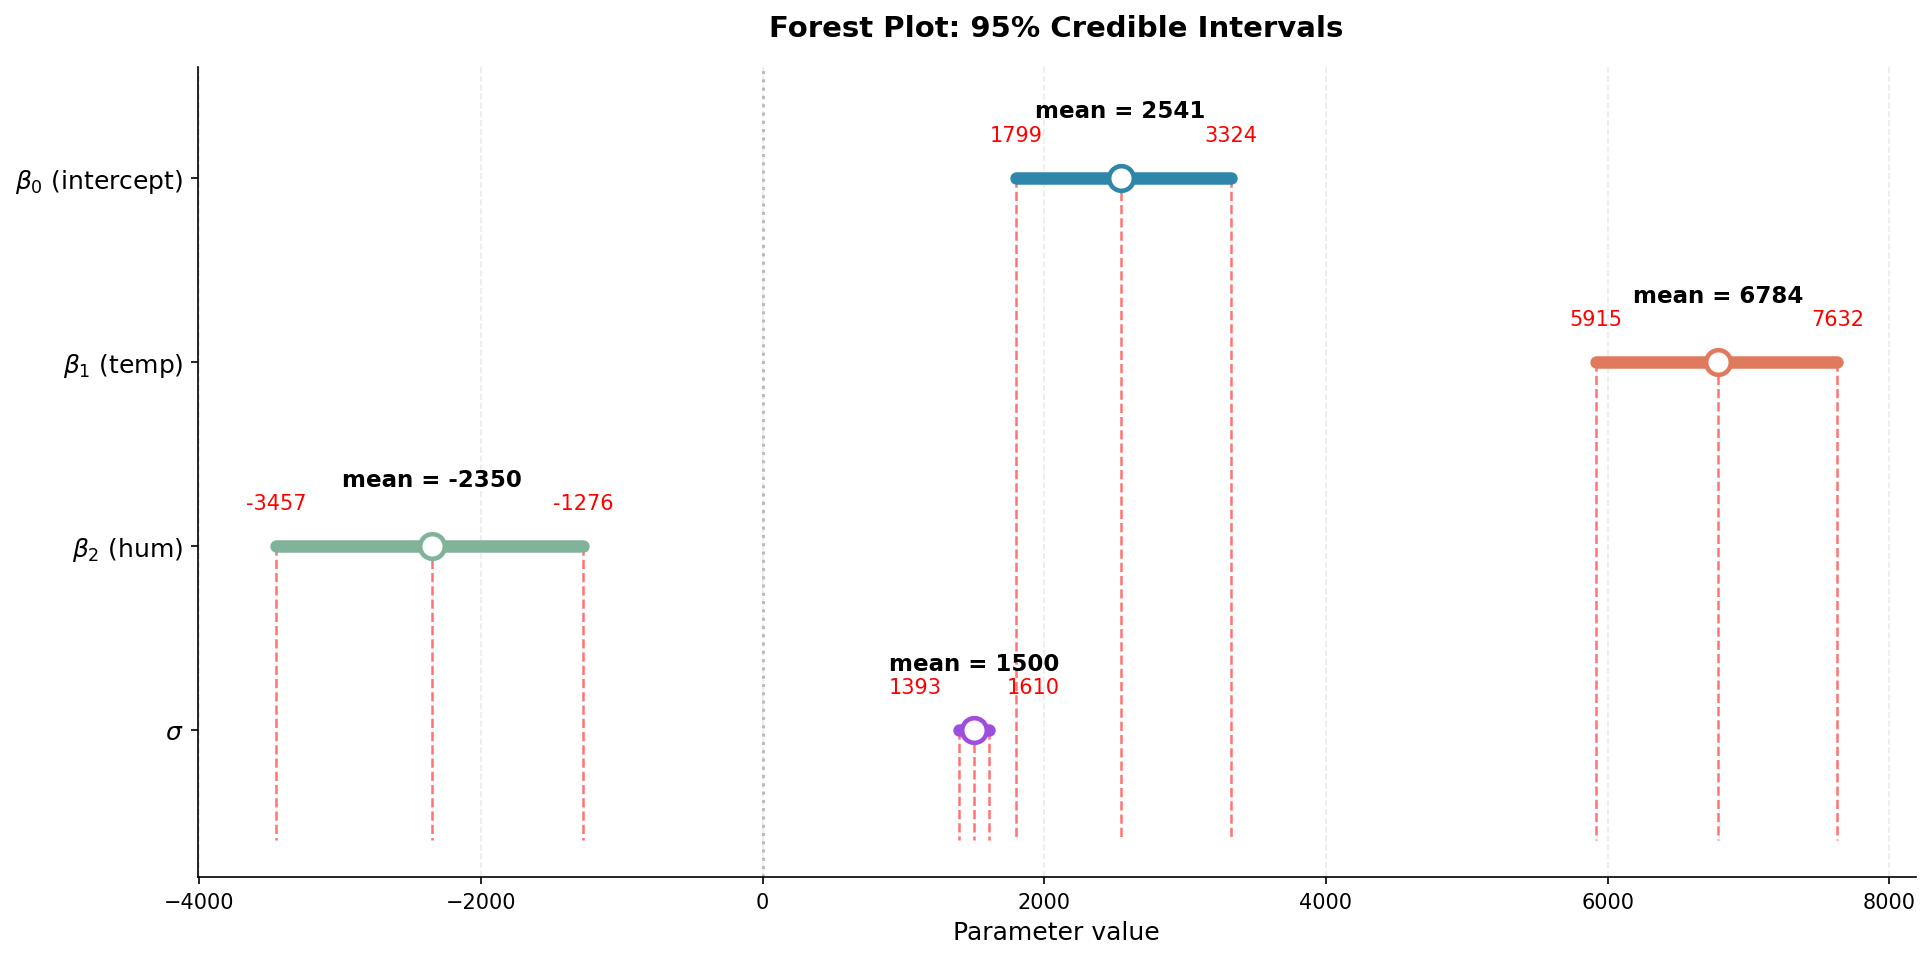
\includegraphics[width=0.85\textwidth]{../results/figures/posterior_forest.png}
    \caption{Forest plot of the posterior 95\% credible intervals. Both $\beta_1$ and $\beta_2$ lie wholly on one side of zero, providing decisive posterior evidence of non-zero temperature and humidity effects on daily rentals.}
    \label{fig:forest}
\end{figure}

\subsubsection{Substantive Interpretation}

Before interpreting the coefficients we recall that, as documented by Module~A in Section~\ref{sec:introduction}, both \texttt{temp} and \texttt{hum} are min--max normalised to the unit interval. The transformation $\texttt{temp} = (T + 8)/47$ for $T \in [-8, 39]\,^{\circ}\text{C}$ and $\texttt{hum} = \text{relative humidity}/100$ implies that coefficient interpretations refer to changes on the normalised scale rather than to raw physical units, and that the meaningful range of each predictor in the data is the full interval $[0, 1]$.

Temperature exerts a substantial positive effect on bike-sharing demand. The posterior mean of $\beta_1$ is $6784$ with 95\% credible interval $(5915,\, 7632)$, so a one-unit increase in normalised temperature is associated, on average, with approximately $6800$ additional daily rentals. Because the credible interval lies wholly above zero --- the lower limit of $5915$ exceeds zero by more than thirteen posterior standard deviations --- the posterior probability that $\beta_1 > 0$ is effectively unity, providing decisive evidence that warmer days are accompanied by markedly higher rental volumes. Translated to the physical scale, the full normalised range $[0, 1]$ corresponds to a temperature swing of $47\,^{\circ}\text{C}$ between the coldest and warmest days in the original dataset; the posterior therefore implies that this swing raises the expected daily rental count by approximately $6800$, identifying temperature as the dominant explanatory mechanism in the present model.

Humidity has a credibly negative effect. The posterior mean of $\beta_2$ is $-2350$ with 95\% credible interval $(-3457,\, -1276)$, indicating that a one-unit increase in normalised humidity is associated, on average, with approximately $2350$ fewer daily rentals; in physical terms, this corresponds to the difference between a perfectly dry and a saturated atmosphere. The exclusion of zero from the credible interval supports the conclusion that humidity meaningfully suppresses bike-sharing activity, in agreement with the negative slope visible in the exploratory scatter plot of Section~\ref{sec:introduction}. The posterior credible interval for $\beta_2$ is somewhat wider than that for $\beta_1$, reflecting both the weaker correlation observed by Module~A and the smaller absolute magnitude of the underlying effect.

The intercept $\beta_0$ has posterior mean $2541$ with credible interval $(1799,\, 3324)$. Because both predictors have been normalised, $\beta_0$ represents the model-implied expected daily rental count when the normalised temperature and humidity are simultaneously zero --- a corner of the predictor space that is not physically attainable in the dataset (it would require near-freezing temperatures together with completely arid air) and is therefore retained for completeness rather than for substantive interpretation.

The residual standard deviation $\sigma$ is estimated very precisely, with posterior mean $1500$ and a narrow 95\% credible interval of $(1393,\, 1610)$. This corresponds to a coefficient of variation of $1500 / 4392 \approx 34\%$ relative to the empirical mean of \texttt{cnt}, indicating that temperature and humidity together leave a substantial proportion of day-to-day variation unexplained. This is consistent with the modest coefficient of determination $R^{2} = 0.405$ reported by Module~A in Section~\ref{sec:frequentist}: a sizeable fraction of the variability in daily rentals reflects calendar effects, holidays, and other meteorological covariates that we have deliberately omitted in order to keep the model focused on the two-predictor specification dictated by the project scope.

\subsubsection{Comparison with the Frequentist Baseline}

A formal comparison of the Bayesian posterior with the OLS estimates of Section~\ref{sec:frequentist} is the subject of Module~A's Section~\ref{sec:frequentist}; here we record only that the posterior means agree with the OLS point estimates to within $1\%$ for all four parameters, and the 95\% credible intervals are nearly indistinguishable in width and location from the corresponding 95\% confidence intervals. This near-coincidence is the expected consequence of our deliberately weakly informative prior: with $n = 360$ observations and prior standard deviations more than an order of magnitude larger than the eventual posterior standard deviations, the likelihood dominates the posterior, and Bayesian point estimates approximate the maximum likelihood estimates to numerical precision. The two paradigms therefore differ here not in their numerical values, but in the interpretation of the resulting intervals --- a distinction discussed by Module~A in Section~\ref{sec:frequentist}.
